% vim: ts=2 sw=2 et :
\documentclass[tikz, border=2mm]{standalone}

\usepackage{times}
\usepackage{txfonts}

\begin{document}
  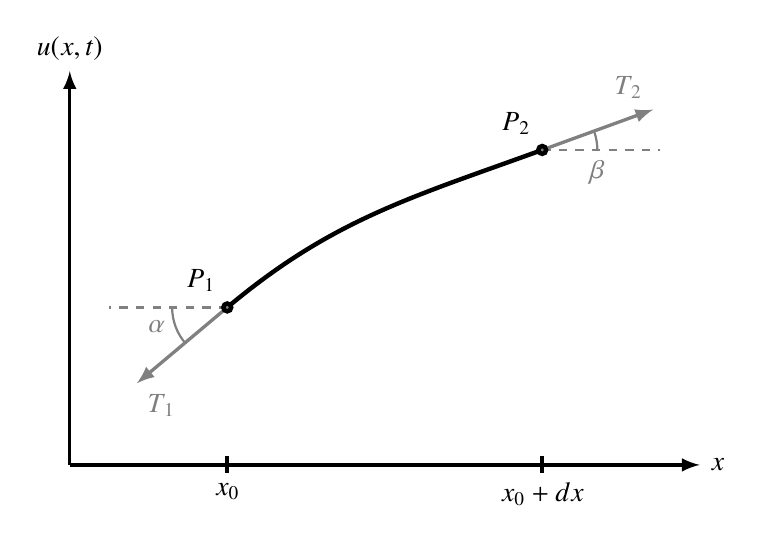
\begin{tikzpicture}[
      axis/.style = {very thick, -latex},
      axis tick/.style = {
        draw, draw = black, fill = black, rectangle,
        inner sep = 0pt,
        minimum height = 2mm,
        minimum width = 1pt,
      },
      string/.style = {
        ultra thick, draw = black,
      },
      string end/.style = {
        string, circle, fill = gray,
        inner sep = 0pt, minimum size = 1mm,
      },
      force/.style = {
        very thick, draw = gray, -latex,
      },
    ]

    % axes
    \draw[axis] (0, 0) -- (8cm, 0) node[right] {$x$};
    \draw[axis] (0, 0) -- (0, 5cm) node[above] {$u(x, t)$};

    % axes ticks
    \node[axis tick, label = {-90:$x_0$}] at (2cm, 0) {};
    \node[axis tick, label = {-90:$x_0 + dx$}] at (6cm, 0) {};

    % string
    \coordinate (A) at (2cm, 2cm);
    \coordinate (B) at (6cm, 4cm);

    \draw[string] (A) to[out = 40, in = 200] (B);

    \draw[force] (A) -- ++(220:15mm) node[gray, below right] {$T_1$};
    \draw[force] (B) -- ++(20:15mm) node[gray, above left] {$T_2$};

    \draw[dashed, gray, thick] (A) -- ++(-15mm, 0);
    \draw[gray, thick] (A) ++ (-7mm,0) arc (180:220:7mm)
      node[midway, left] {$\alpha$};

    \draw[dashed, gray, thick] (B) -- ++(15mm, 0);
    \draw[gray, thick] (B) ++ (7mm,0) arc (0:20:7mm)
      node[pos = 0, below] {$\beta$};

    \node[string end, label={110:$P_1$}] at (A) {};
    \node[string end, label={110:$P_2$}] at (B) {};

  \end{tikzpicture}
\end{document}
